\documentclass{article}
\usepackage[utf8]{inputenc}
\usepackage[english]{babel}
\usepackage{graphicx}
\usepackage{fancyhdr}
\usepackage{array}
\usepackage{hyperref}
\usepackage[figurename=]{caption}
\usepackage{chngcntr}
\counterwithin{figure}{subsection}
\usepackage{ragged2e}



\pagestyle{fancy}
\setlength{\headheight}{52pt}
\fancyhf{}
\rhead{Kumar Shah 2018450045 \\ Prashant Singh 2018450051}
\lhead{Accident Prone Areas Detection}
\rfoot{Page \thepage}
\lfoot{}


\title{Mini Project}
\author{}
\begin{document}
\thispagestyle{empty}
\begin{center}
\textbf{\LARGE Mini Project On \\
\bigskip
Accident Prone Areas Detection\\
\bigskip
By\\
\bigskip
Kumar Shah(2018450045)\\
Prashant Singh(2018450051)\\
}
\bigskip
Under the guidance of\\
\textbf{
\bigskip
\Large Internal Supervisor\\
\LARGE Prof. Harshil T. Kanakia\\
}
\bigskip
\bigskip

\includegraphics[width=5cm]{SPIT-Logo.png}
 \bigskip
 \bigskip
 
\Large Department of Master Of Computer Application\\
Sardar Patel Institute of Technology\\
Autonomous Institute Affiliated to Mumbai University\\

2018-19
\clearpage
\thispagestyle{empty}
\textbf{\Large CERTIFICATE OF APPROVAL\\}
\bigskip
\bigskip
This is to certify that the following students\\
\bigskip
\bigskip
\textbf{
Kumar Shah(2018450045)\\
Prashant Singh(2018450051)\\
}
\bigskip \bigskip
Have satisfactorily carried out work on the project entitled\\
\bigskip \bigskip
\textbf{
\LARGE “Accident Prone Areas Detection”\\
}
\bigskip \bigskip
Towards the fulfilment of project,\\

as laid down by Sardar Patel Institute of Technology during year 2018-19.

\end{center}
\bigskip \bigskip
\begin{flushleft}

\large Project Guide: Prof. Harshil T. Kanakia
\end{flushleft}
\clearpage
\begin{center}
    \thispagestyle{empty}
    \textbf{\Large PROJECT APPROVAL CERTIFICATE\\}
    \bigskip \bigskip
    \large This is to certify that the following students\\
    \bigskip \bigskip \bigskip
    \textbf{
    Kumar Shah(2018450045)\\
    Prashant Singh(2018450051)\\
    }
    \bigskip \bigskip \bigskip
    \large Have successfully completed the Project report on \\ 
    \textbf{\Large“Accident Prone Areas Detection”,}\\
    \large which is found to be satisfactory and is approved\\
    \bigskip \bigskip \bigskip 
    \large At \\
    \bigskip 
    SARDAR PATEL INSTITUTE OF TECHNOLOGY,\\
    ANDHERI (W), MUMBAI.\\
\end{center}
\bigskip \bigskip \bigskip \bigskip \bigskip
\bigskip 
\begin{flushleft}
    INTERNAL EXAMINER
    \hfill
    EXTERNAL EXAMINER
\end{flushleft}
\bigskip \bigskip \bigskip \bigskip \bigskip
\bigskip 
\begin{flushleft}
    HEAD OF DEPARTMENT
    \hfill
    PRINCIPAL
\end{flushleft}
\clearpage

\thispagestyle{empty}
\newpage
\tableofcontents{}
\thispagestyle{empty}
\newpage
\pagenumbering{roman}
\begin{center}
\addcontentsline{toc}{section}{Abstract}
\section*{Abstract}
\begin{flushleft}
\justifying
The rapid growth of technology has made our easier this advancement in technology also increased traffic hazarded. Hence ratio of road accident increases. Most of the Time loss of life due to poor emergency facilities. Our system provide a solution for accident  detection and prevention of human life safety. The application has  been divided into four module based on functionalities. This module is designed to built up and integrated system to cover various aspects of android based Automatic vehicle Accident Detection By Using Android application. The application is designed using location tracking using GPS technology. 
\end{flushleft}
    
    \addcontentsline{toc}{section}{Objectives}
\section*{Objectives}
\begin{flushleft}
    The Application "Help Mate" is used  
         \begin{itemize}
        \item To show accident prone areas.
        \item To provide with navigation.
        \item To alert the user when he passes by accident prone area.
        \item To report an accident and broadcasting to registered mobile numbers.
        \item To report accidents to the Government bodies
        \end{itemize}
\end{flushleft}

\end{center}
\newpage

\addcontentsline{toc}{section}{List Of Figures}
\listoffigures


\addcontentsline{toc}{section}{List Of Tables}
\listoftables
\newpage
\pagenumbering{arabic} 
\setcounter{page}{1}
\begin{flushleft}
    \section{Introduction}
        \subsection{Problem Definition}
        \justifying
        In today's world, accident is one of the major threat in India. Most of people travels by Car or Bike to work. They don't know they may pass by through the accident prone areas (where major accident occurs repeatedly). And there is nothing as such to alert them from accident prone areas.
        Our project (android application) focuses majorly on the same concept i.e., to alert the individual when they pass by any accident prone areas, so that they can avoid accidents in the future.
        \subsection{Objectives and Scope}
        \subsubsection{Objectives}
        The Application "Help Mate" is used  
         \begin{itemize}
        \item To show accident prone areas.
        \item To provide with navigation.
        \item To alert the user when he passes by accident prone area.
        \item To report an accident and broadcasting to registered mobile numbers.
        \item To report accidents to the Government bodies
        \end{itemize}
        \subsubsection{Scope}
        \justifying
        Our System is being made for the identification of the accident prone areas in India.It's main motive is the safety of the travellers in India.In today's world accidents are increasing day by day, our system focuses on reducing them.
        \par
        Our system will generate automatic alert when the user is about to enter the accident prone areas.It will give popup of it as well it will give notification to the user in their phone.Even our system can be used for navigation from one place to another.
        \par 
        In case of emergency and 'Report Accident' button is being kept on the application so as on click on that button it will send the other registered number message that our friend is in trouble.
        
        
        
        \newpage
        \subsection{Existing System}
        Using smartphones to identify road traffic accidents is not a
        new subject. There are completed algorithms for systems
        which utilizes accelerometer as well as GPS to detect vehicle
        accidents using smartphones to detect accidents dates back to
        2011. Because there is already a lot done on this subject, what
        we decided to do was to develop a complete system that is
        more reliable and have much more functionality than the
        existing ones.\\
        Some of the disadvantages of existing system are as follows :
        \begin{itemize}
            \item No Availability \\ There is no such existing system which provides alerts when user passes by an accident prone area.
            \item Limited Features \\ Some of the applications only gives the features such as navigation and guidance
            \item No Automatic Broadcasting \\
            There is no system which provides automatic broadcasting.
            \item No Identification of Accident Prone Areas \\
            There is no such system available for identification of accident prone areas. 
        \end{itemize}
        \newpage
        \subsection{Proposed System}
        \begin{figure}[!ht]
              
              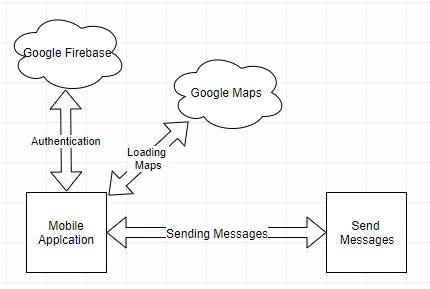
\includegraphics[width=12cm]{ProposedSystem.jpg}
              \renewcommand{\thefigure}{ \thesubsection.\arabic{figure}}
              \caption{ .  Proposed System}
            \end{figure}
        Some of the advantages of our system are as follows :
        \begin{itemize}
            \item User Friendly \\
            It provides attractive interface to the user for guidance and navigation.
            \item Quick Access \\
            Maps can be accessed much faster than other applications.
            \item Informative \\
            Users can easily identify accident prone areas. Also maps are very informative for finding current location and nearby places.
            \item Alerting Users \\
            It alerts users when they pass by any accident prone areas.  
        \end{itemize}
        \newpage
        \subsection{System Requirements}
        \begin{itemize}
            \item Hardware Requirements on Server Side
           \begin{center}
           \begin{table}[!ht]
           \renewcommand\thetable{1.5.1}
               \centering
               \caption{Hardware Requirements on Server Side}
               \label{}
              \begin{tabular}{ | m{5em} | m{7cm} | }
           
            \hline
             Processor & Dual Core Processor or Above  \\ \hline
             RAM & 2GB RAM   \\  \hline
             Storage & 10GB Hard Disk Space for smooth run  \\  \hline
            \end{tabular}
            
           \end{table}
            
            \end{center}
            
            
          \item Hardware Requirements on Client Side 
          \begin{center}
          \begin{table}[!ht]
          \renewcommand\thetable{1.5.2}
              \centering
              \caption{Hardware Requirements on Client Side}
              \label{ }
             \begin{tabular}{ | m{5em} | m{7cm} | }
           
            \hline
             Processor & Dual Core Processor or Above  \\ \hline
             RAM & 512MB RAM   \\  \hline
             Storage & Minimum Hard Disk Space  \\  \hline
            \end{tabular}
              
          \end{table}
            
            \end{center}
            
            
           \item Software Requirements on Server Side
           
           
           \begin{center}
          \begin{table}[!ht]
          \renewcommand\thetable{1.5.3}
              \centering
              \caption{Software Requirements on Server Side}
              \label{"   " }
             \begin{tabular}{ | m{3cm} | m{6cm} | }
           
            \hline
             Operating System & OS Independent  \\ \hline
             Software & Android Studio   \\  \hline
             Database & Firebase   \\  \hline
            \end{tabular}
              
          \end{table}
            
            \end{center}
            
            
            
        \item Software Requirements on Client Side
            \begin{center}
          \begin{table}[!ht]
          \renewcommand\thetable{1.5.3}
              \centering
              \caption{Software Requirements on Client Side}
              \label{"   " "  " }
             \begin{tabular}{ | m{3cm} | m{6cm} | }
           
            \hline
             Operating System & Android OS  \\ \hline
             Android Version & 4.2.2 Or Above   \\  \hline
             Server & Not Required   \\  \hline
            \end{tabular}
              
          \end{table}
            
            \end{center}
            
            
            
            
           
            
            
            \end{itemize}
            
        
        \newpage
    
    \section{Literature Survey}
   The  accident  detection  and  alert  system  provide emergency responders  with crucial  information  at  the earliest possible time. Reducing the time between when an accident  takes place  and when  it is  detected  can reduce mortality  rates.  The  entire  works  have  to  be  integrated with  the  automobile  to  validate  its  functionality  and reliability. Thus this  work will reduce the accident death ratio in considerable  amount even in  roads. Then it has a great importance in day to day life of the people in the  country like  India. This  proposed  work  will  provide vital information about the accidents even in unpopulated area.\\ An automatic accident prevention and reporting system is designed  and  implemented  using GPS modem for finding the location of vehicle in terms of latitude and longitude, as  well  as mobile number for  sending  message  on  mobile  at the receiver end.\\  The  proposed  model  for  accident  detection system  can prove  to  be  an  important  aid  in  constructing  smart transport systems in near future  if implemented properly.  [1]
    \newpage
    
    \section{Software Requirement Specification[SRS] and Design}
        \subsection{Purpose}
        \begin{itemize}
            \item The purpose of this SRS Document is to present a description of project. This SRS outlines the process followed to gather the requirements for the project. This document will also describe how the requirement statements gathered from the stakeholders make their way into features of the system
            \item This document will, in addition, explain the scope, interfaces, and features as well as graphically describe the processes, functions and phases of the Software Development Life-cycle
        \end{itemize}
        \subsection{Definition}
        A software requirements specification (SRS) is a comprehensive description of the intended purpose and environment for software under development. The SRS fully describes what the software will do and how it will be expected to perform. 
        \subsection{Overall Description}
            \subsubsection{Product Functions}
            The product function includes: 
            \begin{enumerate}
                \item Authentication: Users/Admins are required to Sign-up and Log-in. Users can view products and their orders.
                \item Navigation: It helps you to reach from one place to other.
                \item Safety: It will be popup notification if you reach accident prone areas.
                \item One Tap Service: It will let you call the nearby Ambulance Service or any nearby Garages.
                \item Alert System: It will send automated alert or manual alert to the 2-3 registered mobile numbers.
            \end{enumerate}
            
            \subsubsection{User Characteristics}
            There are two types of users: 
            \begin{itemize}
                \item User: User can Sign-up and Login to the app and use it various services.
                \item Admin: Admin can use the services of the Users as well as he even has access to the database.
            \end{itemize}
            
            
        \subsection{Specific Requirement}
            \subsubsection{Functional Requirements}
            \begin{itemize}
                \item The System aims at providing an efficient interface to the user for safety from accident prone areas, it shall also provide the user varied options for contacting a friend at time of accidents. The design is such that the user just have to register once in the application.
                \item The application notifies the user when he reaches nearby accident prone area, it gives notification in the application as well as it even gives pop-up to the user for the same, so the user can avoid accidents.
                \item It also gives additional functionalities of Navigation from one place to another and even it provides broadcasting of message if any emergency occurs in the near future.
            \end{itemize}
            \subsubsection{Non-functional Requirements}
            \begin{enumerate}
                \item Security: The users are required to authenticate themselves before impacting system. It is the facility provided by system to prevent unauthorized access
                \item Availability: The system must be available for access 24 hours, 7 days a week. Also in occurrence of any major malfunctioning, the system should online again as soon as possible. Also system will give the same performance even if many users log-on at the same time.
            \end{enumerate}
            \newpage
            
    \section{Project Analysis and Design}
        \subsection{Methodologies Adapted}
            In Waterfall model, very less customer interaction is involved during the development of the product. Once the product is ready then only it can be demonstrated to the end users.
            \par
            Once the product is developed and if any failure occurs then the cost of fixing such issues are very high, because we need to update everything from document till the logic.
        
            Need of Waterfall Model:
            \begin{itemize}
                \item This model is used only when the requirements are very well known, clear and fixed.
                \item Product definition is stable.
                \item Technology is understood.
                \item There are no ambiguous requirements
                \item Ample resources with required expertise are available freely
                
            \end{itemize}
            \begin{figure}[!ht]
              
              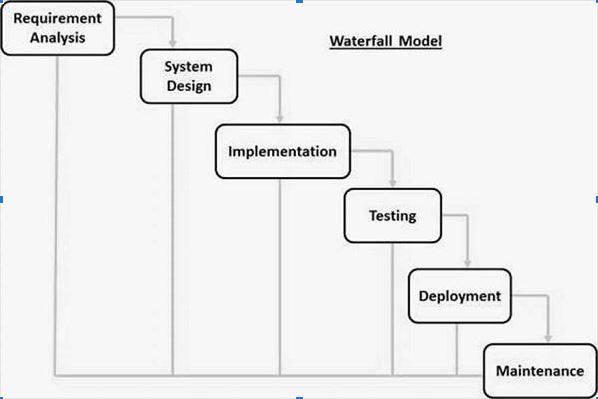
\includegraphics[width=12cm]{WaterfallModel.JPG}
              \renewcommand{\thefigure}{ \thesubsection.\arabic{figure}}
              \caption{ .  Diagrammatic Representation of Waterfall Model}
            \end{figure}
            
            \newpage
        \subsection{Modules}
            \subsubsection{UML Diagram-Use Case Diagram with Report}
            \begin{figure}[!ht]
              
              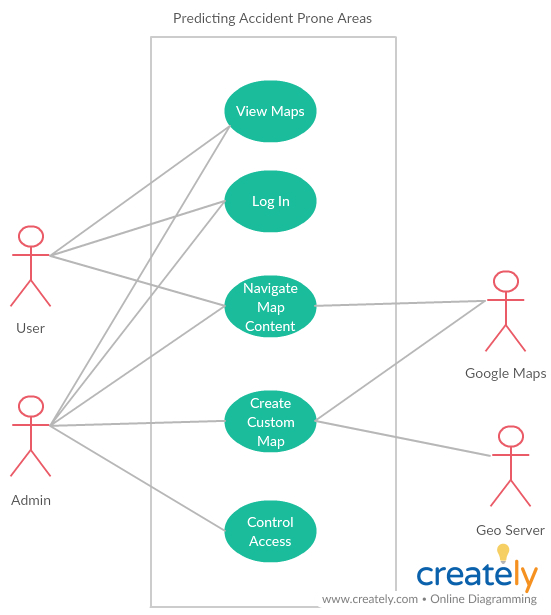
\includegraphics[width=12cm]{UseCase.jpg}
              \renewcommand{\thefigure}{ \thesubsection.\arabic{figure}}
              \caption{ .  Use Case Diagram}
            \end{figure}
            \newpage
            Use Cases:
            \begin{enumerate}
                \item Login
                \item Navigation
                \item Report Accidents
                
                \begin{center}
           \begin{table}[!ht]
           \renewcommand\thetable{4.2.1}
               \centering
               \caption{Use Case Table - Login}
               \label{""""}
              \begin{tabular}{ | m{7em} | m{7cm} | }
           
            \hline
             Use Case ID & 1  \\ \hline
             Use Case Name & Login  \\  \hline
             Actor & User   \\  \hline
            Pre-Condition & They must register themselves first \\ \hline
            Post-Condition & User can use all the features of application\\ \hline
            Flow of events & Register,Login, Access System   \\ \hline
            
            \end{tabular}
           \end{table}
            \begin{table}[!ht]
           \renewcommand\thetable{4.2.2}
               \centering
               \caption{Use Case Table - Navigation}
               \label{""   ""}
              \begin{tabular}{ | m{7em} | m{7cm} | }
           
            \hline
             Use Case ID & 2  \\ \hline
             Use Case Name & Navigation  \\  \hline
             Actor & User   \\  \hline
            Pre-Condition & Login \\ \hline
            Post-Condition & User can reach the destination\\ \hline
            Flow of events & Login,Navigation  \\ \hline
            
            \end{tabular}
           \end{table}
            
            
            
            \begin{table}[!ht]
           \renewcommand\thetable{4.2.3}
               \centering
               \caption{Use Case Table - Report Accident}
               \label{"""  "}
              \begin{tabular}{ | m{7em} | m{7cm} | }
           
            \hline
             Use Case ID & 3 \\ \hline
             Use Case Name & Report Accidents \\  \hline
             Actor & User   \\  \hline
            Pre-Condition & Login \\ \hline
            Post-Condition & Messages will be sent \\ \hline
            Flow of events & Login, Click on Report Accident   \\ \hline
            
            \end{tabular}
           \end{table}
           
           \end{center}
            \end{enumerate}
        \newpage
        \subsection{Database Schema/ Design}
            \subsubsection{E-R diagram}
            \begin{figure}[!ht]
              
              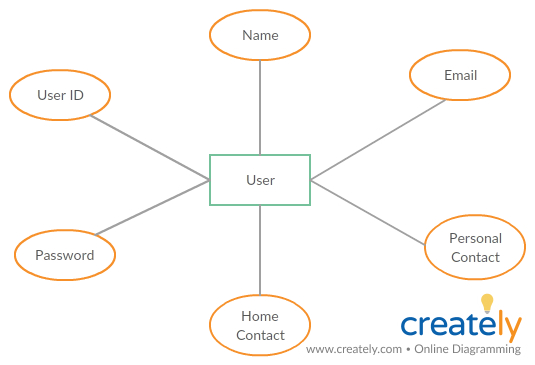
\includegraphics[width=12cm]{ER.jpg}
              
              \caption{ .  ER Diagram}
            \end{figure}
            \newpage
            \subsubsection{Flowchart diagram}
             \begin{figure}[!ht]
              
              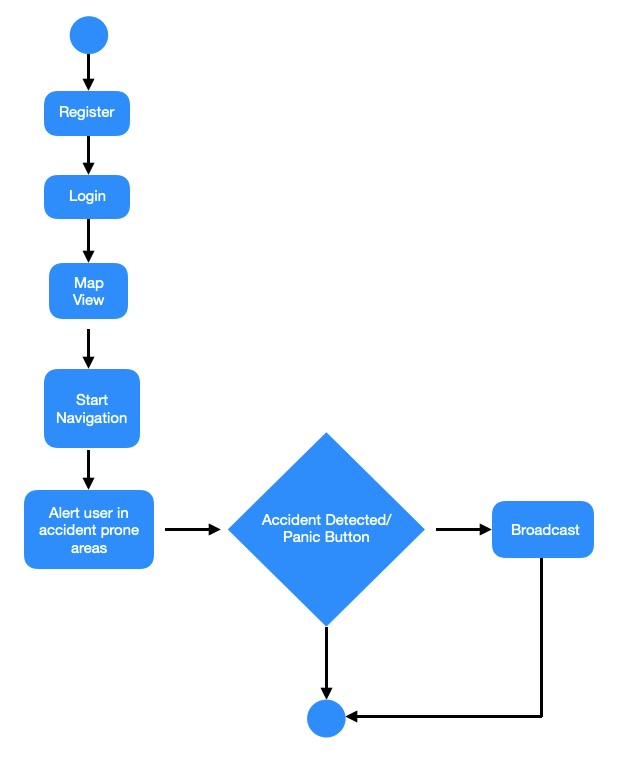
\includegraphics[width=12cm]{FlowChart.jpg}
              \renewcommand{\thefigure}{ \thesubsection.\arabic{figure}}
              \caption{ .  Flowchart Diagram}
            \end{figure}
            \newpage
            \subsubsection{Database Schema Design}
             \begin{figure}[!ht]
              
              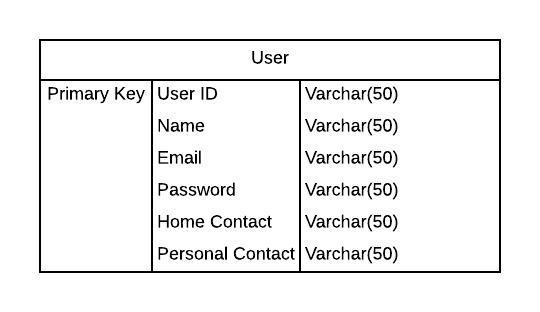
\includegraphics[width=12cm]{DSD.jpeg}
              \renewcommand{\thefigure}{ \thesubsection.\arabic{figure}}
              \caption{ .  Database Schema Design}
            \end{figure}
           
\newpage
            \subsubsection{Work Breakdown Structure}
            \begin{figure}[!ht]
              
              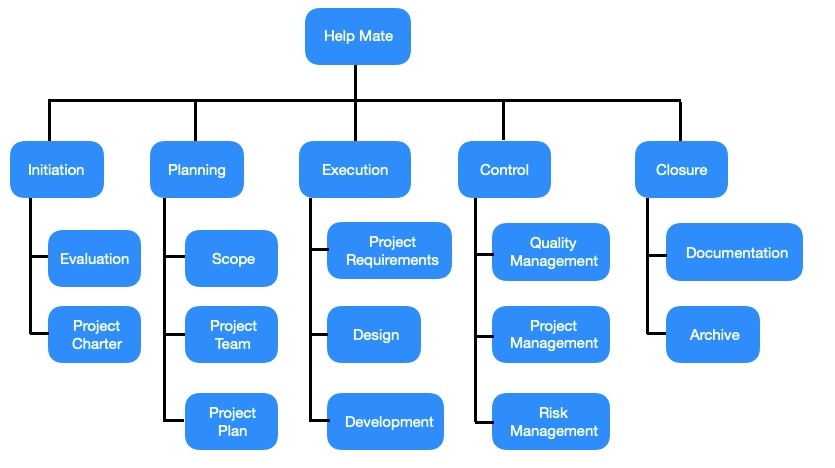
\includegraphics[width=12cm]{WBS.jpg}
              \renewcommand{\thefigure}{ \thesubsection.\arabic{figure}}
              \caption{ .  Work Break Down Structure}
            \end{figure}
            \bigskip
            At the very top of the structure is the project name "Help Mate". This project was divided into 5 phases. They are Initiation, Planning, Execution, Control and Closure. Initiation phase is further divided into Evaluation phase and Project Charter phase. In Planning phase, we discussed Scope, Project Team and Project Plan. In Execution phase, the work done is Project Requirements, Design and Development. In Control Phase, Quality Management, Project Management and Risk Management is being taken care of. In the last phase Closure, Documentation is being made and whole project is being archived.
            
            
            
            
            
            \newpage
            
            \subsubsection{PERT Table}
            \begin{figure}[!ht]
              
              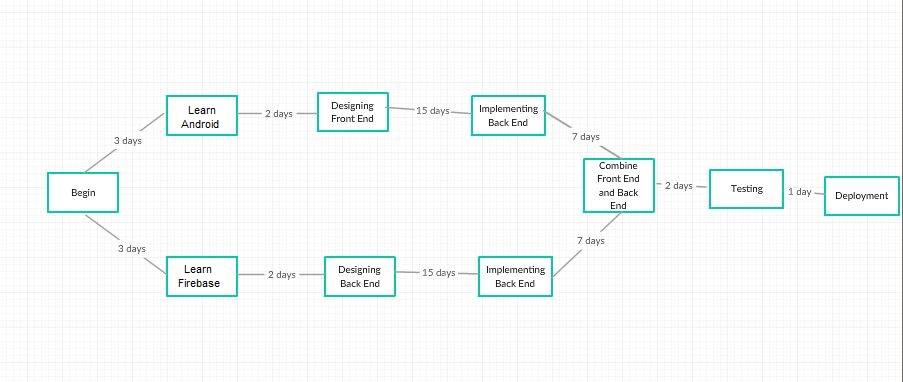
\includegraphics[width=12cm]{Pert.JPG}
              \renewcommand{\thefigure}{ \thesubsection.\arabic{figure}}
              \caption{ .  PERT Table}
            \end{figure}
            

            \subsubsection{Gantt Chart}
            \begin{figure}[!ht]
              
              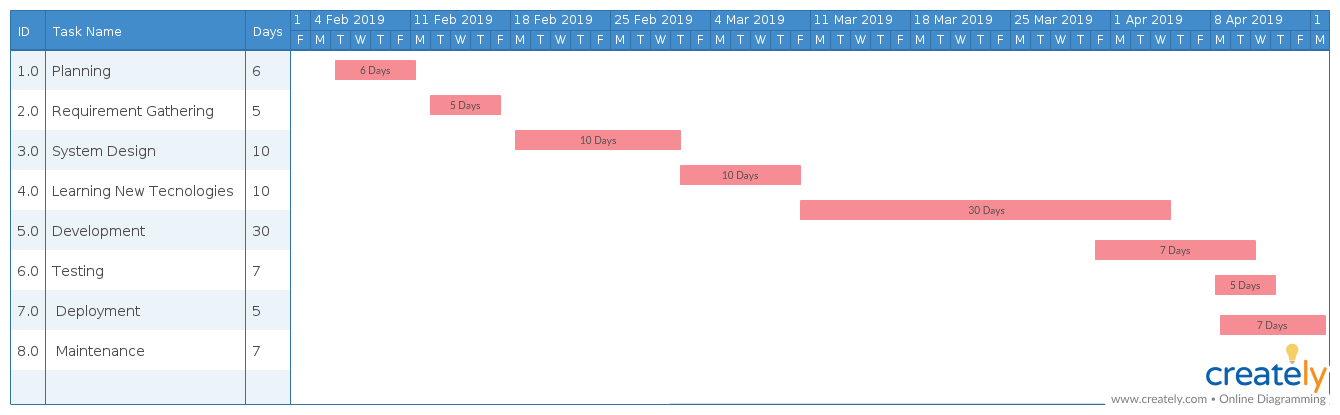
\includegraphics[width=12cm]{GanttChart.jpg}
              \renewcommand{\thefigure}{ \thesubsection.\arabic{figure}}
              \caption{ .  Gantt Chart}
            \end{figure}
            
            \newpage
            
    \section{Project Implementation and Testing}
        \subsection{Snapshot of UI}
      \begin{figure}[!h]
	\centering
	\begin{minipage}[t]{4cm}
		\centering
		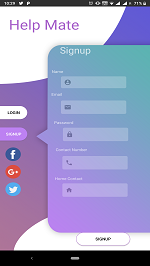
\includegraphics[scale=1]{Signup.png}
		\caption{Signup Page}
	\end{minipage}
	\hspace{3cm}
	\begin{minipage}[t]{4cm}
		\centering
		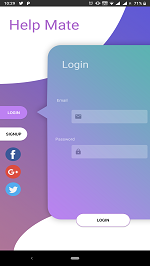
\includegraphics[scale=1]{Login.png}
		\caption{Login Page}
	\end{minipage}
 
	\begin{minipage}[t]{4cm}
		\centering
		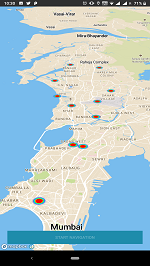
\includegraphics[scale=1]{Maps.png}
		\caption{Maps }
	\end{minipage}
	\hspace{3cm}
	\begin{minipage}[t]{4cm}
		\centering
		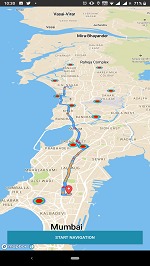
\includegraphics[scale=1]{Navigation.png}
		\caption{Navigation}
	\end{minipage}
	
\end{figure}
            \newpage
            \begin{figure}[!h]
	\centering
	\begin{minipage}[t]{4cm}
		\centering
		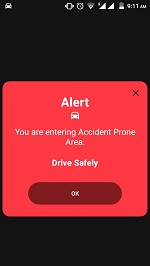
\includegraphics[scale=1]{message1.jpg}
		\caption{Popup Alert}
	\end{minipage}
	\hspace{3cm}
	\begin{minipage}[t]{4cm}
		\centering
		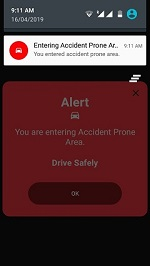
\includegraphics[scale=1]{message2.jpg}
		\caption{Notification}
	\end{minipage}
 
	\begin{minipage}[t]{4cm}
		\centering
		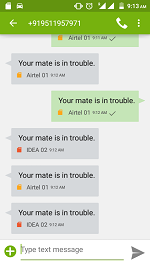
\includegraphics[scale=1]{message3.png}
		\caption{Message Alert}
	\end{minipage}
	
\end{figure}
\newpage
        
        \subsection{Test Cases}
        \begin{center}
           \begin{table}[!ht]
           \renewcommand\thetable{5.2.1}
               \centering
               \caption{Test Case - Login}
               \label{"""}
              \begin{tabular}{ | m{1cm}| m{2cm}| m{2cm}| m{2cm}| m{2cm} | m{1cm} | }
           
            \hline
             Test Case ID & Test Case Name & Test Data & Expected Output & Actual Output & Result  \\ \hline
             1 & User enter email and password & enters the correct email and password & Logged in Successfully & Home Page & Pass  \\  \hline
             2 & User enter email and password & enters the wrong email and password & Prompt error & Prompt error & Pass  \\  \hline
            \end{tabular}
           \end{table}
           \end{center}
           
           \begin{center}
           \begin{table}[!ht]
           \renewcommand\thetable{5.2.2}
               \centering
               \caption{Test Case - Register}
               \label{"""""}
              \begin{tabular}{ | p{1cm}| p{2cm}| p{2cm}| p{2cm}| p{2cm} | p{1cm} | }
           
            \hline
             Test Case ID & Test Case Name & Test Data & Expected Output & Actual Output & Result  \\ \hline
             1 & User enter email and password & valid email and password which doesn't exist in Database & Registered Successfully & Login Page & Pass  \\  \hline
             2 & User enter email and password & Invalid email and password which contains in Database &  Prompt error & Prompt error & Pass  \\  \hline
            \end{tabular}
           \end{table}
           \end{center}
            
            \newpage
    
    \section{Limitations}
    \begin{itemize}
        \item It cannot track you if your location access is off to the user.
        \item If the user's phone is switched off,  he/she cannot be traced, hence our applications fails to send messages to the registered numbers.
        \item If the user does not give message access to the application, it cannot send the message in case of accident.
        
    \end{itemize}
    
    \section{Future Enhancements}
    \begin{itemize}
        \item We can implement automated broadcasting system if the user is in trouble.
        \item Even some other functionalities like giving information about nearby hospitals and garages in case of the accident.
        \item It can even have the tracking features that sends the live location of the user to his family or friends.
    \end{itemize}
    \newpage
    
    \section{User Manual}
        \textbf{Part 1 – Signup }\\
Upon opening the application, user will be greeted with the login screen. If the user has no account,
user can click on signup and register an account. After verification of e-mail id, user’s account will be saved in our database. The user can now proceed
to login.  \\
\newline
\textbf{Part 2 – Login} \\
User needs to enter email first, and then password. If there is an active internet connection, user can proceed to login. \\
\newline
\textbf{Part 3 – Map View} \\
User will be directed to map view. Where he can see all nearby accident prone areas. And can select safe route.
\\
\newline
\textbf{Part 4 – Navigation} \\
User can start navigation in map view. After starting navigation, an alert will be given if user enters any accident prone area. \\
\newline
\textbf{Part 5 – Report Accident} \\
User can report accident during navigation. After reporting accident, message would be broadcasted to all his registered mobile numbers.

    \newpage
    
    \section{References}
    \subsection{References}
    [1.] Patil Ashish and Yadav Abhilash, "Accident Detection System using Android Application", IARJSET , ISSN(Online) 2393-8021, Vol. 4, Special Issue 4, January 2017, PP 118-120 

    
    \subsection{Web References}
    
        [2.] \url{http://staruml.io/}  \newline
        [3.] \url{https://www.creatly.com}
    
    \subsection{Other References}
    
    [4.] Head First Android Development: A Brain-Friendly Guide \newline [Dawn Griffiths, David Griffiths] 
    \newpage
            
    
\end{flushleft}
\end{document}